% ECE578 Project
% Bliss Brass, Kai Brooks, Tyler Hull, Mikhail Mayers, Roman Minko
% Fall 2019

% Document settings ------------------------------------------------
\documentclass[a4paper,12pt]{article}

\newcommand{\figOverlay}{\put(34,10){\color{black!50} \figWatermark}} % Figure overlay settings
\newcommand{\figWatermark}{}%\small Brooks \today} 		% Figure overlay text
\newcommand{\figHere}{\begin{overpic}[percent,scale=0.32]}	% Settings for all figures
\newcommand{\figHereB}{\begin{overpic}[percent,scale=2]}	% Settings for all figures
\newcommand{\figHereC}{\begin{overpic}[percent,scale=0.5]}	% Settings for all figures

\newcommand{\authorname}{Brass, Brooks, Hull, Mayers, Minko}
\newcommand{\classnumber}{ECE578}
\newcommand{\projectname}{Mice and Cheese}

% Packages ------------------------------------------------

\usepackage[USenglish]{babel} 	% American English
\usepackage{blindtext}			% Generate latin crap
\usepackage[yyyymmdd]{datetime} % Sets date format to ISO 8601 standard
\renewcommand{\dateseparator}{-}% Sets date format to ISO 8601 standard

\usepackage{graphicx}			% Image importing and display
\graphicspath{ {images/} }		% Path to image folder
\usepackage{xcolor}				% Allows normal color words
\usepackage{color, colortbl}


\usepackage{float}				% Adds 'H' for figure placement location
\usepackage{enumitem}			% Use for QandA environment
\usepackage{booktabs}			% Merging columns in tables

\usepackage[nostamp]{draftwatermark}	% use [nostamp] when finished, [firstpage] otherwise
\SetWatermarkText{DRAFT}
\SetWatermarkColor{red!50}
\SetWatermarkScale{3}


\usepackage{overpic}				% Puts text over figures
\usepackage[american]{circuitikz}	% American-style circuit diagrams

\usepackage{amsmath}				% Multi-line equations
\usepackage{caption}				% Equation caption formatting
\usepackage{physics}				% Easier derivatives
\usepackage{gensymb}				% Enable \degree for degree symbol
\usepackage{siunitx}				% SI units

\usepackage{hyperref}				% makes links
\usepackage[normalem]{ulem}			% adds strikethrough

\usepackage{array}					% Used for centering tabular data
\newcolumntype{M}[1]{>{\centering\arraybackslash}p{#1}} % The actual centered column format

\usepackage{listings} %For code in appendix

% background image for the first page
\usepackage{eso-pic}
\newcommand\BackgroundPic{%
\put(0,0){%
\parbox[b][\paperheight]{\paperwidth}{%
\vfill
\centering
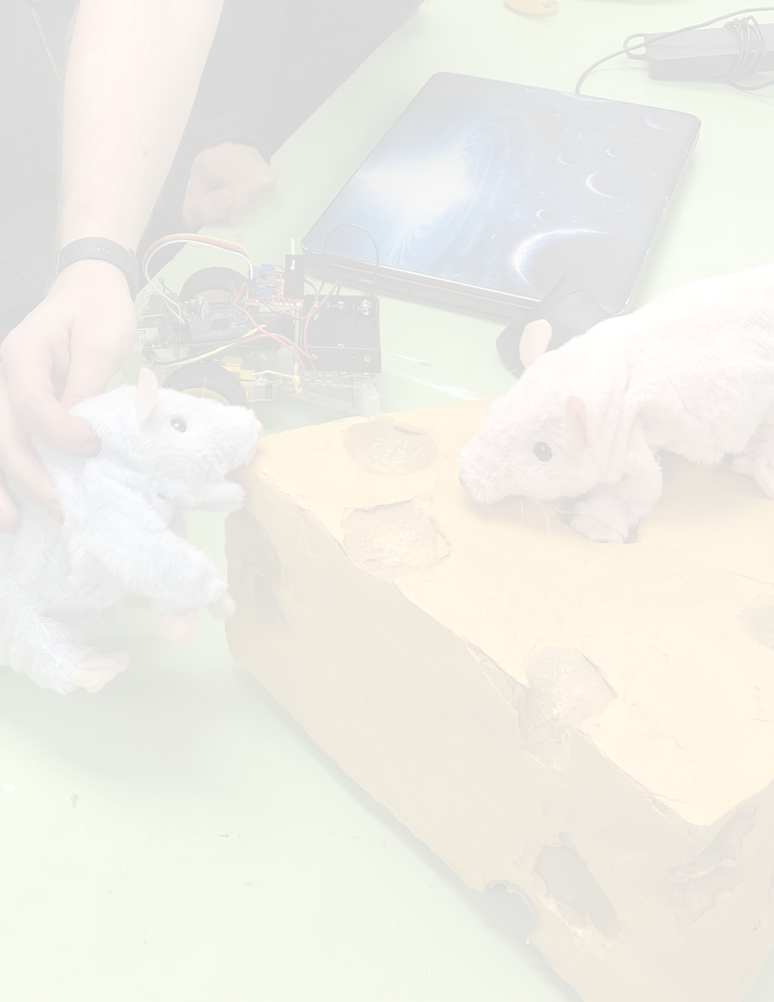
\includegraphics[width=\paperwidth,height=\paperheight]{images/bg.png}%
\vfill
}}}

\definecolor{mymauve}{rgb}{0.58,0,0.82}
\definecolor{mygreen}{rgb}{0,0.6,0}
\definecolor{mygray}{rgb}{0.5,0.5,0.5}
\definecolor{ltgray}{rgb}{0.937, 0.937, 0.956}	% Divide standard RGB values by 255 for some reason 

% PSU colors
\definecolor{PSUgreen}{RGB}{106,127,16}
\definecolor{PSUltgreen}{RGB}{168,180,0}
\definecolor{PSUblue}{RGB}{0,117,154}
\definecolor{PSUltblue}{RGB}{161,216,224}
\definecolor{PSUgray}{RGB}{71,67,52}
\definecolor{PSUbrown}{RGB}{96,53,29}
\definecolor{PSUsienna}{RGB}{163,63,31}
\definecolor{PSUred}{RGB}{210,73,42}
\definecolor{PSUorange}{RGB}{220,155,50}
\definecolor{PSUyellow}{RGB}{230,220,143}
\definecolor{PSUtan}{RGB}{232,221,162}
\definecolor{PSUpurple}{RGB}{101,3,96}


\newenvironment{QandA}
	{\begin{enumerate}[label=\arabic*.]\sl} % Use slanted question text and Arabic numerals
  {\end{enumerate}}
\newenvironment{answered}{\par\normalfont}{} % Paragraph break and use normal font

% fancy header / footer lines
\usepackage{fancyhdr}% http://ctan.org/pkg/fancyhdr
\pagestyle{fancy}% Change page style to fancy
\fancyhf{}% Clear header/footer
\fancyhead[L]{\textcolor{PSUgray}{\classnumber}}
\fancyhead[R]{\textcolor{PSUgray}{\projectname}}
\fancyfoot[L]{\textcolor{PSUgray}{\authorname}}
\fancyfoot[R]{\textcolor{PSUgray}{\thepage}}
\renewcommand{\headrulewidth}{0.4pt}% Default \headrulewidth is 0.4pt
\renewcommand{\footrulewidth}{0.4pt}% Default \footrulewidth is 0pt


% Title Page ------------------------------------------------
\begin{document}
\AddToShipoutPicture*{\BackgroundPic} % add background image to title page

% Formatting for code in appendix; why it's right here, nobody knows
\lstset { 
  language=Matlab,
  basicstyle=\footnotesize\ttfamily,
  numbers=left,
  stepnumber=1,
  showstringspaces=false,
  tabsize=1,
  breaklines=true,
  breakatwhitespace=false,
  stringstyle=\color{mymauve},
  keywordstyle=\color{blue},
  commentstyle=\color{mygreen}, 
}

\begin{titlepage}
	\begin{center}
		\vspace*{1cm}

		\huge\textsc{\textcolor{mygray}{\sout{Police and Thief}}}\\
		\huge\textsc{\projectname}

		\vspace{0.5cm}
		\small\textsc{\classnumber}
		
		\vspace{1.5cm}
		\normalsize \authorname 
		
		\vspace{0.5cm}
		%Lab TA: N/A
		
		\vfill
		\vspace{0.8cm}
		
		
\includegraphics[width=0.5\textwidth]{images/psulogo_horiz_msword_cd.png}
		
		\vspace{0.5cm}
		Electrical and Computer Engineering\\
		Portland State University\\
		\today
		 
	\end{center}
\end{titlepage}

% Table of contents ------------------------------------------------
\newpage
\tableofcontents


% Begin paper ------------------------------------------------
\newpage
\pagenumbering{arabic}

\section{Overview}
	As a new design scheme, we changed the \textit{Policemen and Thief} to the less violent, \textit{Mice and Cheese}.\\

	Design a game with 3 ``Viking Bots": two dressed as mice and the third as a wedge of cheese. The goal of the game is to keep the cheese away from the hungry maws of the two little mice. The game uses object recognition to find the location of each game piece on the board. The program builds a game board and determines the proper strategy so that the agents can move effectively in the right direction. The user goes first and can control the course of the cheese, and the mice will continuously move towards the cheese after each turn. Will the cheese escape the mice? Or will it get eaten? Tune in and find out next time on Perkowski’s comedy cartoon hour.

\section{Hardware}
	The hardware for our project consists of 3 robots and all their associated parts. In the past, this project utilized two Viking Bots and a single, more massive hexapod robot. Our requirements for the project were to replace the hexapod robot with another Viking Bot and to improve the robustness of the hardware. This would ensure that our hardware can run more consistently, at a faster pace, and in more diverse conditions than were possible in previous implementations of the project.

\subsection{Goals}
	\begin{enumerate}
		\item Purchase and assemble a new Viking Bot
		\item Assess what hardware was left over from previous implementations of project
		\item Upgrade and standardize battery packs for all robots
		\item Improve wiring reliability and cable management
		\item Ensure that the robots can run consistently at top speed for fast gameplay	
	\end{enumerate}

\subsection{Design}
	We assembled our project’s robot cars from an inexpensive kit, which was quick to assemble.  The Viking Bot robot kit consists of the following parts: 
	\begin{itemize}
		\item An acrylic sheet with mounting holes and cutouts for wires
		\item A set of two DC motors and wheels
		\item A swivel caster for a back wheel
		\item A battery pack (AA battery size)
		\item An L298N H-Bridge Module
		\item A Raspberry Pi microprocessor board
	\end{itemize}

	Due to the nature of using a ``kit" robot, we didn’t have a lot of latitude to design the hardware we were using. However, we undertook the development of a better battery and power management system for the robots after discovering the following problems:

	\begin{itemize}
		\item Batteries we inherited had differing voltages, causing robots to function differently from one another
		\item Some robots used multiple battery packs to achieve uniform voltages, adding extra weight to the robot
		\item The $V_{IN}$ port powered the Raspberry Pi's, causing damage to the boards.
		\item H-Bridge modules were providing inconsistent outputs and current limiting the Raspberry Pi's
	\end{itemize}
	
	To solve these problems, we designed a rechargeable battery and power system using three 18650 batteries that provided a stable voltage for the motors and Raspberry Pi. This design increased our run time, avoided damage to the Raspberry Pi's, and was easier to implement across all three robots.
	
\subsection{Implementation}
	Initially, we were told by a member of the previous team that their principal concern was using non-identical battery packs. This irregularity caused one of the robots to turn more quickly than the other. Also, we knew that we were replacing the hexapod robot with a Viking Bot, which required ordering a new robot kit and assembling it.

\subsection{Assess Project Hardware}
	Our first task was to assess what hardware the previous team left. Unfortunately, the robots we found in the old project locker were in a sad state. The locker included all sorts of batteries, servos, screws, electronics, and other parts in a large pile. The two Viking Bot robots we inherited had loose jumper wires and tape all over them. There were three types of battery packs in the locker for the robots: a USB pack (too low voltage for constant use), AA battery packs (not rechargeable), and a sizable Li-Po battery pack (no charger available). We were not able to test any of the hardware since we did not have a battery of the correct voltage that we could recharge. These irregularities left us in the position of needing to correct the power issues immediately so we could test the robots. In order to correct the mess in the locker and to avoid losing vital parts, we cleaned out all the components. We organized them by type into labeled boxes. This organization has significantly improved the storage locker and made the project run more smoothly.
	
	\begin{figure}[H]	 		
		\centering
	  	\label{fig:}
	  	\figHere{images/organized_locker.jpg} \figOverlay
	  	\end{overpic}
	  	\caption{Organized locker}
	\end{figure}
	
	\begin{figure}[H]	 		
		\centering
	  	\label{fig:}
	  	\figHere{images/battery_box.jpg} \figOverlay
	  	\end{overpic}
	  	\figHere{images/box_of_servoParts.jpg} \figOverlay
	  	\end{overpic}
	  	\caption{Battery and servo parts}
	\end{figure}
	
	
\subsection{Battery and Power System}

	After learning that the Viking Bots use the L298N H-Bridge module for powering the motors and the Raspberry Pi, we were able to determine that we needed to be able to provide close to 12V for the system. Additionally, the robots were set up to use the 5V output from the H-Bridge module to power the Raspberry Pi. However, after inspection of the L298N schematic, we discovered two problems with this setup:
	
	\begin{itemize}
		\item The L298N requires a separate 5V power supply if supplying the module with more than 12V in order to protect the H-Bridge chip.
		\item The 5V onboard voltage regulator for 5V output (L78M05) can only supply up to 0.5A of current on the output.
	\end{itemize}

	Therefore, using a battery pack that is greater than 12V requires a different power supply for obtaining 5V. Initially, this was our only consideration, and we purchased rechargeable batteries in the 18650 size for the system. We selected these batteries their high mAh ratings and high current output ability. Then, we purchased battery holders, batteries for all the robots, and a battery charger. Using three batteries in series produces $3.7V \cdot 3 = 11.1V$ nominal voltage for the system. However, when fully charged, these batteries can reach 4.2V and provide 12.6V to the system, potentially damaging the onboard voltage regulator and the Raspberry Pi.

	In addition, the Raspberry Pi requires up to 2.5A for peak power. This requirement is 2A over the maximum available from the onboard voltage regulator supply. Due to this rating, we needed to find a different solution for powering the Raspberry Pi in order to provide a stable voltage with enough amperage to function safely.

	\begin{figure}[H]	 		
		\centering
	  	\label{fig:}
	  	\figHereB{images/L298N_schematic.jpg} \figOverlay
	  	\end{overpic}
	  	\caption{Schematic}
	\end{figure}
	
	Our solution was to add a separate voltage regulator that adjusts to the correct voltage for the Raspberry Pi and provides enough amperage for it to run without brownouts or damage to the board. We chose the DROK adjustable voltage regulator for this task as we could tune them to precisely 5V with the potentiometer on the underside, and they can handle up to 3A (0.5A over the Raspberry Pi’s max requirements).
	
	\begin{figure}[H]	 		
		\centering
	  	\label{fig:}
	  	\figHere{images/voltage_regulator_closeup.jpg} \figOverlay
	  	\end{overpic}
	  	\caption{Voltage regulator}
	\end{figure}
	
	\begin{figure}[H]	 		
		\centering
	  	\label{fig:}
	  	\figHere{images/hBridge_closeup.jpg} \figOverlay
	  	\end{overpic}
	  	\caption{H-Bridge module}
	\end{figure}
		
\subsection{Building the Third Viking Bot}
	Assembling the robot kit was very straight forward. The kit contained instructions and required only a screwdriver to assemble. Building a new Viking Bot from scratch allowed us to understand better how to make improvements to the wiring and set up to make the robot more robust. 
	
	\begin{figure}[H]	 		
		\centering
	  	\label{fig:}
	  	\figHere{images/New_vikingBot.jpg} \figOverlay
	  	\end{overpic}
	  	\figHere{images/car_assembly.jpg} \figOverlay
	  	\end{overpic}
	  	\caption{Robot kit fully assembled with H-Bridge module}
	\end{figure}
	
	We standardized the setup of the robots, putting the battery pack over the back swivel wheel for better weight distribution. We mounted the H-Bridge between the motors underneath the deck, the Raspberry Pi at the front, and the voltage regulator between it and the battery pack. We also attached a power switch for each robot to save on battery life. Finally, we used shrink wrap for solder connections to avoid short circuits. Then we zip-tied wires to the chassis paying close attention to keeping them out of the way. We mounted major components using velcro for ease of access. Later, we added each robot’s IP address to the bottom for easy identification.
	
		\begin{figure}[H]	 		
		\centering
	  	\label{fig:}
	  	\figHere{images/car_top_view2.jpg} \figOverlay
	  	\end{overpic}
	  	\figHere{images/car_underside.jpg} \figOverlay
	  	\end{overpic}
	  	\caption{Finished robot with robust wiring and updated power system}
	\end{figure}
	
	\begin{figure}[H]	 		
		\centering
	  	\label{fig:}
	  	\figHereC{images/Updated_rasp-l298n_bb.jpg} \figOverlay
	  	\end{overpic}
	  	\caption{Final wiring diagram for Viking Bots}
	\end{figure}
		

\subsection{Fixing damaged Raspberry Pi's}
	When our battery packs first arrived, we were still attempting to utilize the 5V regulator on the H-Bridge modules. However, when we attempted to power on the robots, we discovered that one of the Raspberry Pi’s we inherited was not powering on. We then tried using our own Raspberry Pi in the system, and it immediately started smoking and was damaged.

	After investigating the cause of the issue, we determined that the 5V regulator on the H-Bridge module was damaged. This regulator was causing some increased current draw or voltage spike that fed into the Raspberry Pi. Since the system was set up to feed power to the Pi through the VIN pin, there was no protection on the circuit, and it fried the diode that typically protects the Raspberry Pi. We assume that the H-Bridge’s voltage regulator became damaged from being supplied with more than 12V as the system under test had been using the higher-rated Li-Po battery during the previous iteration.

	This situation was what prompted us to switch to a dedicated voltage regulator for the Pi, but it left us without a control board for the robots. After inspecting the other non-working pi we inherited, we saw that it too had damage to the diode. Thankfully we were able to order more diodes and replace them. This diode reinstallation fixed the boards and allowed us to use them for the robots. However, we still had an issue with using the VIN pin as it was not protected.

	\begin{figure}[H]	 		
		\centering
	  	\label{fig:}
	  	\figHere{images/Diode_replacement.jpg} \figOverlay
	  	\end{overpic}
	  	\caption{Diode replaced just above the Micro USB port}
	\end{figure}
		
	We cannibalized three micro USB cables to get power from our new voltage regulators and send it into the power port of the Raspberry Pi. To do this, we cut and stripped the USB cable and found the V+ and V- wires with a multimeter. After finding these, we wired them to the correct lines on the voltage regulator output, then plugged the micro-USB into the Raspberry Pi power port. This solution gave us multiple layers of protection against more voltage issues.

\subsection{Building an Enclosure for the Robots}
	During the project, we realized the need for an additional task in the hardware category. One of our robots needed an enclosure in order for our cameras to differentiate it from the others during training. We decided that the project would transition from police chasing a thief to rats chasing cheese. So we needed to develop and cheese-like enclosure that was light enough for the Viking Bot to be still able to move quickly.

	Our initial thought was to purchase a foam Green Bay Packers “Cheesehead” hat and modify it for our project. Unfortunately, due to time constraints and availability, we were not able to get one in time for this to work. We instead decided to try to create a custom enclosure ourselves. 

	A trip to the hardware store yielded some purple insulation sheets, gorilla glue, and yellow spray paint. The next step was to trace out a cheese wedge on the sheets, then cut out four of them, like a layer cake. After making a rough cut of the shape, a smaller template was made using a sheet of bamboo. This bamboo template was then taped to each rough cut piece of foam and used as a cut guide through a hot wire foam slicer. 

	\begin{figure}[H]	 		
		\centering
	  	\label{fig:}
	  	\figHere{images/foam_sheets.jpg} \figOverlay
	  	\end{overpic}
	  	\figHere{images/cheese_template_guide.jpg} \figOverlay
	  	\end{overpic}
	  	\caption{Foam sheets and bamboo template}
	\end{figure}
		
	Next, the bottom two wedges had the center removed to make space for the robot electronics and wheels. We cut slots between these two sheets to make space for bamboo mounting brackets for attaching to the robot. We glued the sheets together, clamped the lot of them, and left it to dry. After the glue dried, we used a heat gun to melt classic holes into the cheese for a more recognizable look. Then, we used plastic wood putty to smooth out any differences between the sheets and to add some texture to the enclosure. We repeated this process three times to ensure reliable putty coverage, and then spray painted the entire thing yellow. Lastly, we mounted the robot inside.
	
	\begin{figure}[H]	 		
		\centering
	  	\label{fig:}
	  	\figHere{images/cheese_holes.jpg} \figOverlay
	  	\end{overpic}
	  	\figHere{images/cheese_spread.jpg} \figOverlay
	  	\end{overpic}
	  	\caption{Foam wedge with melt spots and wood putty}
	\end{figure}
	
	\begin{figure}[H]	 		
		\centering
	  	\label{fig:}
	  	\figHere{images/cheese.jpg} \figOverlay
	  	\end{overpic}
	  	\figHere{images/cheese_w_wheels.jpg} \figOverlay
	  	\end{overpic}
	  	\caption{Finished cheese wedge from top and side view}
	\end{figure}
	
	We ordered rat stuffed animals for the enclosures of our other Viking Bots. The original plan was to order rats that were large enough to un-sew and wrap around our robots. With this in mind, we ordered the most enormous stuffed rats we could find within our price range, which ended up being a length of 19 inches. However, upon their arrival, we learned that they included the tail in the length measurement, and the tails were quite long. That meant that we did not quite have enough space to wrap them around the robots, so we decided to mount them to the top of the robots instead, like rats piloting the Viking Bots.\\

	We ordered two white rats, but we soon realized that we should make them different colors so the vision model could recognize them more easily. To accomplish this, we attempted to use grey and brown fabric dye to give the rats a darker color. However, the dye had an unusual reaction to the fabric of our rats. After washing and drying, the ``grey" rat turned blue, and the ``brown" rat turned pink. Still, this provided enough difference for us to feel comfortable training the vision model with them.
	
	\begin{figure}[H]	 		
		\centering
	  	\label{fig:}
	  	\figHere{images/dyeing_rat2.jpg} \figOverlay
	  	\end{overpic}
	  	\caption{White rat getting ready for dyeing}
	\end{figure}
	
	\begin{figure}[H]	 		
		\centering
	  	\label{fig:}
	  	\figHere{images/dyeing_rat.jpg} \figOverlay
	  	\end{overpic}
	  	\figHere{images/dyeing_rat4.jpg} \figOverlay
	  	\end{overpic}
	  	\caption{Hand-dying to avoid dunking}
	\end{figure}

	\begin{figure}[H]	 		
		\centering
	  	\label{fig:}
	  	\figHere{images/rat_roman2.jpg} \figOverlay
	  	\end{overpic}
	  	\figHere{images/rats_on_cheese2.jpg} \figOverlay
	  	\end{overpic}
	  	\caption{Rats on Roman and rats on cheese}
	\end{figure}
	
		\begin{figure}[H]	 		
		\centering
	  	\label{fig:}
	  	\figHere{images/car_w_bluRat.jpg} \figOverlay
	  	\end{overpic}
	  	\figHere{images/car_w_pinkRat.jpg} \figOverlay
	  	\end{overpic}
	  	\caption{Blue and pink rats mounted on robots}
	\end{figure}

\subsection{Challenges}
	\begin{itemize}
		\item The complete disarray of the project equipment in the locker introduced much confusion as we tried to determine what we needed to fix and what we needed to order. This chaos resulted in us spending more money to order parts and way more time than we anticipated just assessing what was available to us and what was working.
		\item A member from the previous group initially told us that everything was up and running and just needed battery replacement and assorted electrical fixes. This miscommunication further added to the confusion while getting started and resulted in us not understanding the actual state of the project right away. Overall, it wasted a large chunk of our time.
		\item Our battery holders came with wire rated for fewer amps than we needed. During our initial test, we used the H-Bridge that we did not know was faulty. This problem caused an increased current draw and ended up melting a battery pack wire and almost blowing up the battery. This situation caused us to think very carefully about how we should improve the power system on the robots.
		\item Frying the diodes on the Raspberry Pi was a significant setback for us. We were not able to test multiple robots until we had more controllers set up. We were able to order new parts and replace the diodes quickly, so we did not waste too much time on this.
		\item Figuring out what the previous group built with the wiring was a big challenge, as well. There were no diagrams or schematics for the wiring left over from the last team. We had to deal with different types of batteries, taped connections, strange switch setups, and daisy-chained jumper wires that were all contributing to inconsistent results.
		\item Correcting the hardware issues and making the system more robust took far more time than we had allocated for it. We were under the impression that the hardware was all working and needed minor adjustments. Instead, it required us to rebuild it completely. This issue meant we had a lot less time than we thought to work on computer vision and game concepts than we originally planned.
	\end{itemize}

\subsection{Future improvements}
	\begin{itemize}
		\item A shield board for the Raspberry Pi, so wires use either screw terminals or solder connections instead of jumper wires.
		\item A better H-Bridge module that allowed for powering the Raspberry Pi without the need for an additional voltage regulator.
		\item Larger motors could replace the current versions to get increased torque and speed.
		\item Different wheels with softer tires would make an excellent addition to getting better traction on slick floors.
		\item Laser cutting a smaller deck for the robots would allow us to fit the rats to over the top for better aesthetics.
		\item If we use a standalone voltage regulator, we can upgrade the 18650 battery pack size to a four-battery holder version for even longer runtime. This change would also provide extra power for adding sensors or cameras to the robots.
	\end{itemize}

\section{Movement}
	Each Viking Bot has a Raspberry Pi that sends signals to an L298N H-Bridge. We created the controls using simple python functions that send commands which control the direction, power, and speed of the motors. It is possible to sign into the board remotely and send instructions using the wifi capabilities of the Raspberry Pi.

\subsection{Goals}
	\begin{itemize}
		\item Control each robot remotely
		\item Control speed, timing, and direction of robots
		\item Streamline all hardware to allow identical control schemes for each robot
	\end{itemize}

\subsection{Design}
	The Viking Bots are functionally Braitenberg vehicles. The control is simple and sent to the H-Bridge via the Raspberry Pi. We control the movement of the robots by the applied power and the direction of the motor’s rotation. The robots are fundamentally simple but need a mechanism to control them remotely.

\subsection{Implementation}
	The Viking Bots are feedback-driven agents that we control through the overall game program. The user gives the program instructions in which way they want the bots to move. The program interprets this command and decides the turn direction and motor-driven distance.

\subsection{Challenges}
	The lack of documentation regarding movement is a considerable challenge. The primary control program on each robot is simple and easy to follow; however, the mechanics of the game and functionality have been the biggest hurdle. 
	\begin{itemize}
		\item No documentation
		\item No instructions for game use
		\item No instructions on setup
		\item No comments in code
	\end{itemize}

\subsection{Planned Improvements}
	\begin{itemize}
		\item Better documentation
		\item Example or walkthrough of how to set up a game
		\item Inline code comments explaining how each function operates
	\end{itemize}
	
	
\section{Vision}
\subsection{Introduction}
	The vision module allows the Viking Bots to take whatever information they have around them in their environment and implement it into the software. The software used for the vision portion and in preparation for training was OpenCV (open-source computer vision and machine learning library), MATLAB programming language, Darknet (open-source neural network framework), YOLO (real-time object detection system), YOLO Mark (GUI for marking bounded boxes of objects in images for training neural network Yolo). We use all these packages in preparation and integration of the training.

\subsection{Goals}
	\begin{enumerate}
		\item Determine how we want to set up the game board
		\item Set up the camera at an angle where it will capture the whole game board
		\item Take images of the robots on each one of the tiles that make up the game board
		\item Generate text files for each image containing the coordinates of each robot
		\item Write a program that generates permutations of each image and the text files along with them
		\item Add the images and text files into Darknet for training
	\end{enumerate}

\subsection{Design}
	We stuck with using the same design method as the previous group that worked on this project, with some modifications and the addition of the MATLAB program. We changed the Hexapod to another Viking Bot for faster mobility. We also designed and created costumes for each robot to make it easier for object detection. The computer differentiates the rats by color, and the cheese looks strikingly different on its own. These modifications required us to re-train the machine vision algorithm.

\subsection{Implementation}
	In order to train the robots, we needed images of the robots on the game board, as well as text files containing coordinates of each robot. The process for this required us to set up the game board and camera, as it would be set up for the demonstration. The game board is made up of 16 triangle tiles that are connected to make up one giant triangle.\\

	We began taking images of the robots on the game board. We needed to make sure to have images of each robot being in each of the small triangle tiles. Another essential approach was taking pictures of the robots on each tile from different angles. We decided to rotate the robots 45 degrees in each small triangle tile and capture pictures of all angles of the robots. We also took images of the robots being obstructed by other robots to train the neural network for those kinds of situations.\\

	Once we captured all of the images (201 images), we used a GUI called Yolo\_Mark to create bounding boxes around each robot in each image to generate text files for the coordinates of each robot. As mentioned before, training requires these text files.\\

	In order to improve accuracy for training, Kai wrote a program in Matlab that generated permutations of each image. This program reduces issues in detecting robots. Some permutations adjusted the coordinates of the robots, so the MATLAB program.\\

\subsection{MATLAB and permutation training}
	The associated MATLAB r2018a file generates permutations of all images in the training folder, such as color-shifting, adding grain, de-noising, and rotating. These permutations ensure the training algorithm learns to identify the robots in sub-optimal conditions, or learns to identify them more fundamentally. For example, adding noise to the image requires more advanced line-recognition. Rotating the images forces the algorithm to understand what the robots look like from different angles, for instance, if future groups set up the webcam differently. Color-shifting forces the algorithm to learn more about the shape and structure of the robots, instead of a simple color-matching.\\
	
	The program also copies and outputs the associated text files, so it is imperative that the text files of the training (input) pictures already exist from Yolo\_Mark. User-adjustable settings, such as the number of permutations per image, have labels at the beginning of the program.\\
	
	While none of these are technically necessary to train the algorithm, training using permutated images results in more consistent identification in suboptimal environments.\\
	
	Note that we used MATLAB arbitrarily as a quick way to generate permutations without needing to set up various Python-related virtual environments and manage external dependencies. There is no practical reason why permutations require MATLAB specifically.

\section{Useful Links}
Link to GIT repository: \href{https://github.com/mmayers88/Robotics}{https://github.com/mmayers88/Robotics}\\

OpenCV installation: \href{https://docs.opencv.org/3.4.7/d7/d9f/tutorial_linux_install.html}{https://docs.opencv.org/3.4.7/d7/d9f/tutorial\_linux\_install.html}\\

Darknet/YOLO: \href{https://github.com/AlexeyAB/darknet}{https://github.com/AlexeyAB/darknet}\\

YOLO training - \href{https://medium.com/@manivannan_data/how-to-train-yolov3-to-detect-custom-objects-ccbcafeb13d2}{https://medium.com/@manivannan\_data/how-to-train-yolov3-to-detect-custom-objects-ccbcafeb13d2}\\

Yolo\_Mark: \href{https://github.com/AlexeyAB/Yolo_mark}{https://github.com/AlexeyAB/Yolo\_mark}\\

\section{Major Purchases}
	\begin{table}[H]
	\centering
		\begin{tabular}{|M{.3\textwidth}|M{.3\textwidth}|M{.3\textwidth}|} % Col width
		\hline
		\textbf{Item} & \textbf{Cost} & \textbf{Date Received} \\ \hline
		Battery Charger (Universal Smart Battery Charger 4 Bay by Eastshine) & \$27.95 & 2019-10-10  \\ \hline		
		Battery Holders (6 pcs 3 x 3.7V 18650 by Sackorange) & \$6.99 & 2019-10-10  \\ \hline	
		Spare Robot Car (Perseids DIY Robot Smart Car) &  \$13.99 & 2019-10-16  \\ \hline			
		Motor Driver (L298N) & \$6.89 & 2019-10-16  \\ \hline			
		18650 Batteries (Samsung 25R 18650 2500mAh 20A) & \$28.05 & 2019-10-15  \\ \hline	
		4x Voltage Dividers (12V to 6V Converter and Regulator by DROK) & \$39.96 &  \\ \hline			
		NETGEAR AC750 Dual Band WiFi Router & \$39.88 &  \\ \hline			
				
		\end{tabular}						
		\caption{Itemized purchases}	
	\end{table}
	
	\section{Darknet training flowchart}
		\begin{figure}[H]	 		
		\centering
	  	\label{fig:}
	  	\figHereC{images/training_flowchart.png} \figOverlay
	  	\end{overpic}
	  	\caption{Flow chart for training machine vision}
	\end{figure}


	\section{MATLAB code of image permutator}
	\lstinputlisting[language=Matlab]{code/imagePerm_68406b5911fa9689330d8ce4011daac789b97487.m}

	\section{Python code for main function}
	\lstinputlisting[language=Python]{code/main.py}

	

\end{document}